\chapter{Creating Reports}\label{rmarkdown}

Every serious scholar dreams of recording their knowledge in a leather-bound tome
that will lie forgotten and dusty on the shelves of an out-of-the-way library
at a small college with a dubious reputation
until someone naïve enough to believe that they can control forces beyond mortal ken
stumbles upon it and unleashes ravenous horrors to prey upon the sanity of the innocent.
Sadly,
in these diminished times we must settle for dry expositions of trivia
typeset in two columns using demure fonts and sequentially-numbered citations.

But there is hope.
One of R's greatest strengths is a package called \texttt{knitr}
that translates documents written in a format called R~Markdown into HTML, PDF, and e-books.
R~Markdown files are a kind of programmable document:
authors can interleave prose with chunks of code in R (or other languages)
and \texttt{knitr} will run those chunks to create tables and diagrams
as it processes the document.
To aid this,
the RStudio IDE includes tools to create new documents,
insert and run code chunks,
preview documents' structure and output,
and much more.

That's the good news.
The bad news is that Markdown itself isn't a standard:
it is instead a set of ad hoc implementations flying in loose formation.
While basic elements like headings and links are more or less the same in R~Markdown
as they are in (for example) \gref{g:gfm}{GitHub Flavored Markdown},
people who have used other dialects may trip over small differences.

This chapter starts by introducing Markdown and a simple publishing workflow,
then shows how to embed code and customize reports.
We close by showing how to publish reports on GitHub,
which offers free hosting for small websites.

\section{How can we create and preview a simple page?}

To begin,
create a file called \texttt{first.Rmd} and add the following text to it:

\begin{lstlisting}
## Methods {-}

Something *really important*.

An [external link](https://r4py.tech).

[Another link][rstudio]

<!-- link table below -->

[rstudio]: https://rstudio.com
\end{lstlisting}

This shows several key features of Markdown:

\begin{itemize}
\item
  A level-1 heading (\texttt{h1} in HTML) is put on a line starting with \texttt{\#}.
  A level-2 heading (\texttt{h2}) would use two of these and so on.
\item
  Putting \texttt{\{-\}} immediately after the heading title suppresses numbering.
  This is one of R~Markdown's extensions to Markdown.
\item
  Paragraphs are separated by blank lines.
\item
  Text can be enclosed in single asterisks for \emph{italics}
  or double asterisks for \textbf{bold}.
\item
  To create a link,
  put the visible text in square brackets
  and the URL in parentheses immediately after it.
  This is the reverse of HTML's order,
  which puts the URL inside the opening \texttt{a} tag
  \emph{before} the contained text that is displayed.
\item
  Links can also be written by putting text inside square brackets
  and an identifier immediately after it,
  also in square brackets.
  Those identifiers can then be associated with links in a table at the bottom of the page.
\item
  Comments are enclosed in \texttt{{\textless}!-{}-} and \texttt{-{}-{\textgreater}} as they are in HTML.
\end{itemize}

\begin{figure}[h]
  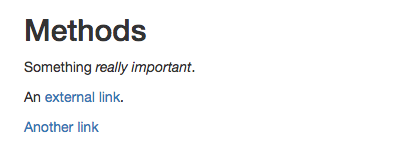
\includegraphics{figures/rmarkdown/first-page.png}
  \caption{Our First Page}
  \label{fig:first-page}
\end{figure}

Figure~\ref{fig:first-page} shows what the HTML corresponding to our simple Markdown document looks like.
To preview it,
go to the mini-toolbar at the top of your document in the RStudio IDE
and click ``knit''
to call the appropriate function from \texttt{knitr}
(Figure~\ref{fig:knit-button}).
We will see later and in the exercises how to knit documents ourselves.

\begin{figure}[h]
  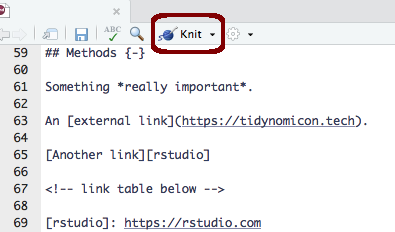
\includegraphics{figures/rmarkdown/knit-button}
  \caption{Knit Me}
  \label{fig:knit-button}
\end{figure}

\section{How can we run code and include its output in a page?}

If this was all R~Markdown could do,
it would be nothing more than an idiosyncratic way to create HTML pages.
What makes it powerful is the ability to include code chunks
that are evaluated as the document is knit
and whose output is included in the final page.
Put the lines below in a file called \texttt{second.Rmd}:

\begin{lstlisting}
Displaying the colors:

```{r}
colors <- c('red', 'green', 'blue')
colors
```
\end{lstlisting}

The triple back-quotes mark the start and end of a block of code;
putting \texttt{\{r\}} immediately after the back-quotes at the start
tells \texttt{knitr} to run the code
and include its output in the generated page,
which therefore looks like Figure~\ref{fig:second-page}.

\begin{figure}[h]
  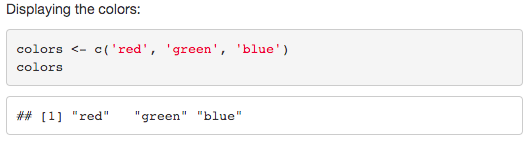
\includegraphics{figures/rmarkdown/second-page.png}
  \caption{Our Second Page}
  \label{fig:second-page}
\end{figure}

\begin{quote}
\textbf{Knitting Selectively}

We don't have to execute all of the code in a document every time we knit:
the \texttt{Code} pulldown in RStudio's main menu offers a variety of ways
to run regions of code.
The IDE also gives us a keyboard shortcut to insert a new code chunk,
so there really is no excuse for not making notes as we go along.
\end{quote}

We can put any code we want inside code blocks,
and can control execution and formatting
by putting options inside the curly braces at the start of the code block:

\begin{itemize}
\item
  \texttt{\{r\ label\}} gives the chunk a label that we can cross-reference.
  Labels must be unique within documents,
  just like the \texttt{id} attributes of HTML elements.
\item
  \texttt{\{r\ include=FALSE\}} tells \texttt{knitr} to run the code
  but \emph{not} to include either the code or its output in the finished document.
  While the option name is confusing---the code is actually included in processing---this
  is handy when we have setup code that loads libraries or does other things
  that our readers probably don't care about\footnote{Though every block of code we don't show
    makes our work slightly less reproducible.}.
\item
  \texttt{\{r\ eval=FALSE\}} displays the code but doesn't run it,
  and is often used in tutorials like this one.
\item
  \texttt{\{r\ echo=FALSE\}} hides the code but includes the output.
  This is often used for displaying static images
  as we will see below.
\end{itemize}

These options can be combined by separating them with commas,
which leads to documents like this:

\begin{lstlisting}
# My Thesis {-}

```{r setup, include=FALSE}
# Load tidyverse but don't display messages.
library(tidyverse)
```

```{r read-data, message=FALSE}
earthquakes <- read_csv('earthquakes.csv')
```

A profound quotation to set the scene.
And then some analysis:

```{r calculate-depth-by-magnitude}
depth_by_magnitude <- earthquakes %>%
  mutate(round_mag = round(Magnitude)) %>%
  group_by(round_mag) %>%
  summarize(depth = mean(Depth_Km))
  depth_by_magnitude
```

Now let's visualize that:

```{r plot-depth-by-magnitude, fig.height=2}
depth_by_magnitude %>%
  ggplot() +
  geom_point(mapping = aes(x = round_mag, y = depth))
```
\end{lstlisting}

In order:

\begin{itemize}
\item
  The document title is a level-1 header with suppressed numbering.
\item
  The first code chunk is called \texttt{setup}
  and neither it nor its output are included in the output page.
\item
  The second chunk is called \texttt{read-data}.
  It is shown in the output,
  but its output is not.
\item
  There is then a very short paragraph.
\item
  The third code chunk calculates the mean depth by rounded magnitude.
  Both the code and its output are included;
  the output is just R's textual display of the \texttt{depth\_by\_magnitude} table.
\item
  After an even shorter paragraph,
  there is another named chunk whose output is a plot rather than text.
  \texttt{knitr} runs \texttt{ggplot2} to create the plot and includes it in the page.
  (We explicitly set the figure's height with \texttt{figsize=2} so that it will fit in this book.)
\end{itemize}

When this page is knit,
the result is as shown in Figure~\ref{fig:third-page}.

\begin{figure}[h]
  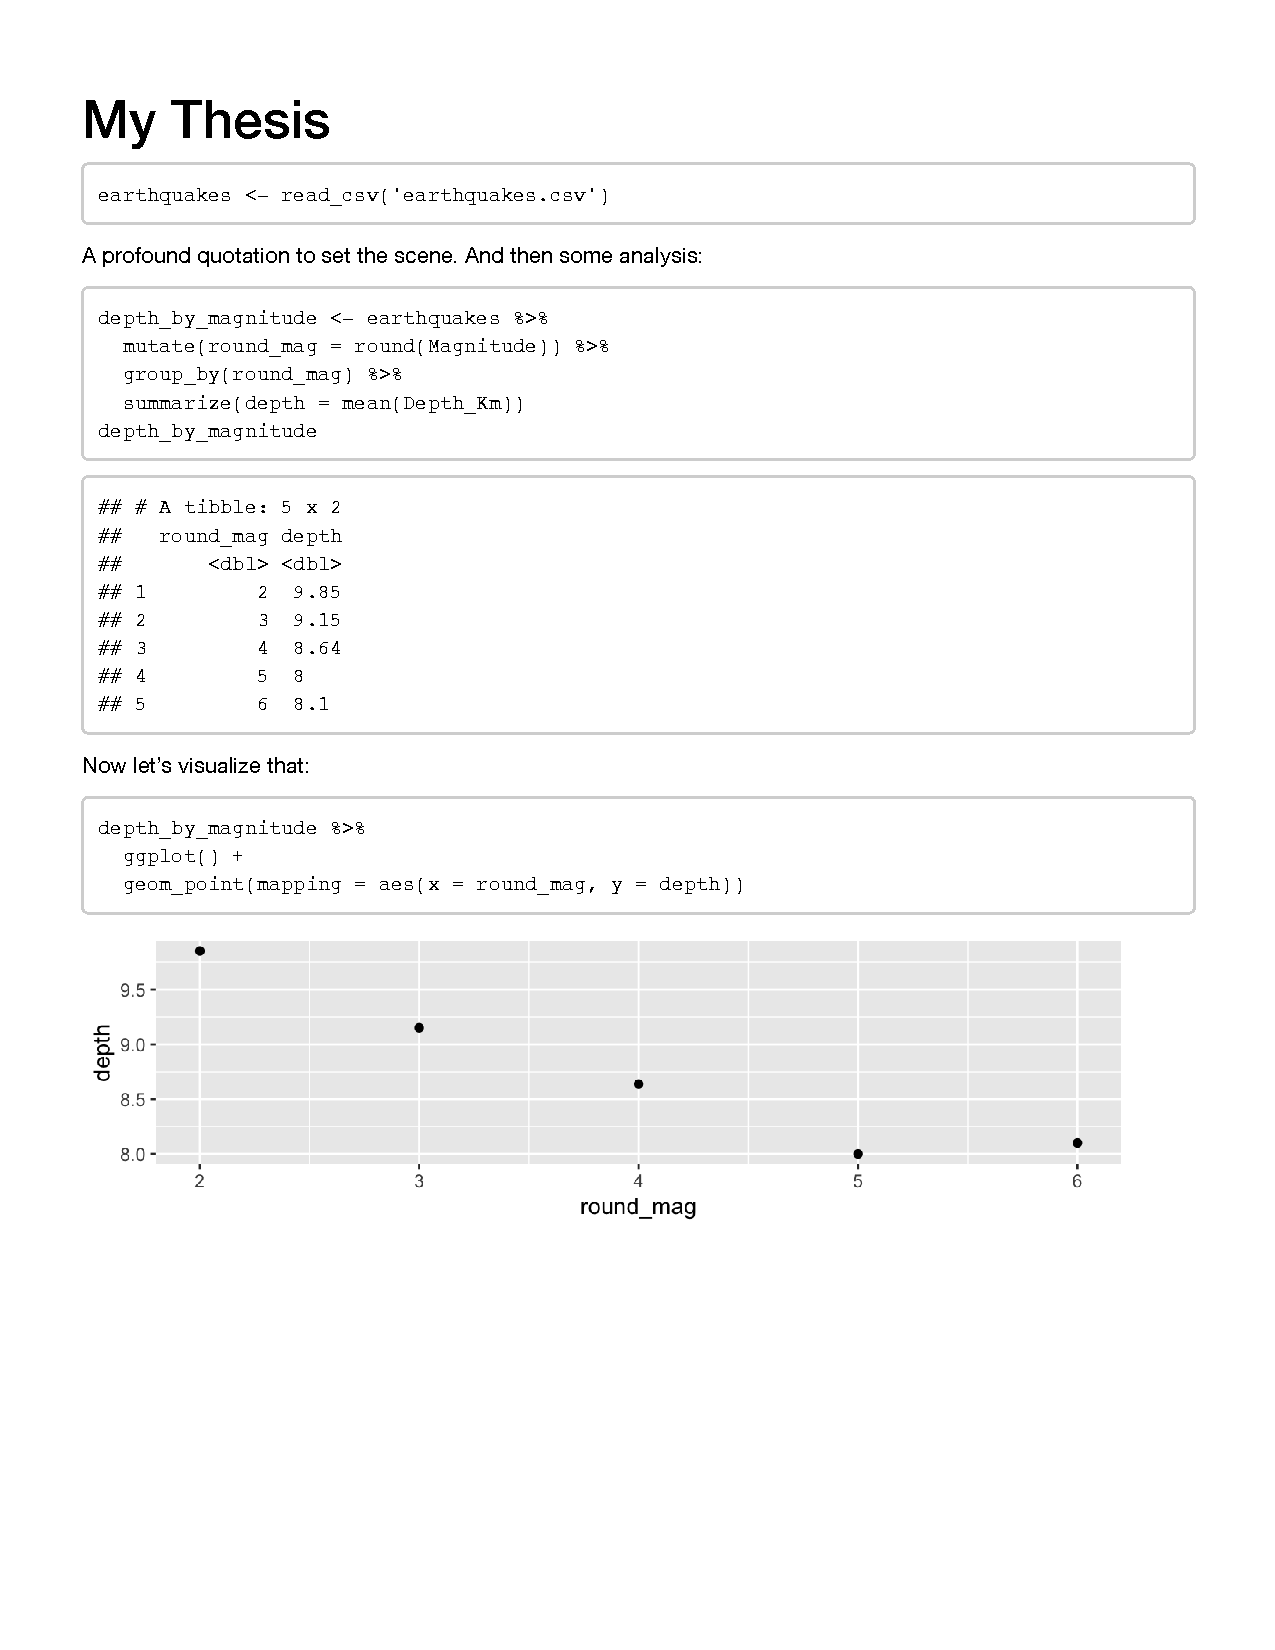
\includegraphics{figures/rmarkdown/third-page.pdf}
  \caption{Our Third Page}
  \label{fig:third-page}
\end{figure}

If we want to include a static image such as a screenshot in a report,
we can use Markdown's own syntax:

\begin{lstlisting}
```markdown
![Summoning Ritual](figures/summoning-ritual.jpg)
```
\end{lstlisting}

or create an R code chunk with a call to \texttt{knitr::include\_graphics}:

\begin{lstlisting}
```{r summoning-ritual, echo=FALSE, fig.cap='Summoning Ritual'}
knitr::include_graphics('figures/summoning-ritual.jpg')
```
\end{lstlisting}

The options for the latter give the code chunk an ID,
prevent it from being echoed in the final document,
and add a caption.
While using a code block requires a bit more typing than a simple Markdown image inclusion,
it allows us to select different images based on the type of document we are creating.
For example,
if we want to include an SVG version of a diagram in HTML
but need a PDF when using LaTeX,
we can use make the choice like this:

\begin{lstlisting}
if (knitr::is_latex_output()) {
  knitr::include_graphics('figures/web/diagram.pdf')
} else {
  knitr::include_graphics('figures/book/diagram.svg')
}
\end{lstlisting}

\section{How can we format tables in a page?}

Tables are the stalwart cornerstone of data science.
While they are not as showy as their graphical counterparts,
they permit closer scrutiny
and are accessible both to people with visual challenges
and to the machines whose eventual triumph over us
will usher in an algorithmic age free of superstition and mercy.

The simplest way to format tables in R~Markdown is to use \texttt{knitr::kable}:

\begin{lstlisting}
earthquakes <- read_csv('earthquakes.csv')
earthquakes %>%
  head(5) %>%
  kable()
\end{lstlisting}

\begin{tabular}{l|r|r|r|r}
\hline
Time & Latitude & Longitude & Depth\_Km & Magnitude\\
\hline
2016-08-24 03:36:32 & 42.6983 & 13.2335 & 8.1 & 6.0\\
\hline
2016-08-24 03:37:26 & 42.7123 & 13.2533 & 9.0 & 4.5\\
\hline
2016-08-24 03:40:46 & 42.7647 & 13.1723 & 9.7 & 3.8\\
\hline
2016-08-24 03:41:38 & 42.7803 & 13.1683 & 9.7 & 3.9\\
\hline
2016-08-24 03:42:07 & 42.7798 & 13.1575 & 9.7 & 3.6\\
\hline
\end{tabular}

Our output is more attractive if we install and load the \texttt{kableExtra} package
and use it to style the table.
We must call its functions \emph{after} we call \texttt{kable()},
just as we call the styling functions for plots after \texttt{ggplot()}.
Below,
we select four columns from our earthquake data and format them as a narrow table
with two decimal places for latitude and longitude,
one for magnitude and depth,
and some multi-column headers:

\begin{lstlisting}
earthquakes %>%
  select(lat = Latitude, long = Longitude,
         mag = Magnitude, depth = Depth_Km) %>%
  head(5) %>%
  kable(digits = c(2, 2, 1, 1)) %>%
  kable_styling(full_width = FALSE) %>%
  add_header_above(c('Location' = 2, 'Details' = 2))
\end{lstlisting}

\begin{table}[H]
\centering
\begin{tabular}{r|r|r|r}
\hline
\multicolumn{2}{c|}{Location} & \multicolumn{2}{c}{Details} \\
\cline{1-2} \cline{3-4}
lat & long & mag & depth\\
\hline
42.70 & 13.23 & 6.0 & 8.1\\
\hline
42.71 & 13.25 & 4.5 & 9.0\\
\hline
42.76 & 13.17 & 3.8 & 9.7\\
\hline
42.78 & 13.17 & 3.9 & 9.7\\
\hline
42.78 & 13.16 & 3.6 & 9.7\\
\hline
\end{tabular}
\end{table}

\section{How can we share code between pages?}

If we are working on several related reports,
we may want to share some code between them.
The best way to do this with R~Markdown is to put that code in a separate \texttt{.R} file
and then load that at the start of each document using the \texttt{source} function.
For example,
all of the chapters in this book begin with:

\begin{lstlisting}
```{r setup, include=FALSE}
source('common.R')
```
\end{lstlisting}

By convention the chunk is named \texttt{setup},
and neither it nor its output are displayed.
All it does is load and run \texttt{common.R},
which contains:

\begin{lstlisting}
library(tidyverse)
library(reticulate)
library(rlang)
library(knitr)

knitr::opts_knit$set(width = 69)
\end{lstlisting}

The first four lines load libraries that various chapters depend on;
the last one tells \texttt{knitr} to set the line width to 69 characters,
which affects how output is broken to fit a printed page.

\section{How can we parameterize documents?}

\texttt{knitr} has many other options besides line width,
and the tools built on top of it
like \href{https://bookdown.org/yihui/blogdown/}{Blogdown} and \href{https://bookdown.org/}{Bookdown}
have many more.
Rather than calling functions to set these options' values,
you can and should add a header to each document.
If we use \texttt{File...New\ File...RMarkdown} to create a new R~Markdown file,
it initially looks like this:

\begin{lstlisting}
---
title: "fourth"
author: "Greg Wilson"
date: "2020-01-21"
output: html_document
---
\end{lstlisting}

\begin{enumerate}
\item
  The header starts with exactly three dashes on a line of their own and ends the same way.
  A common mistake is to forget the closing dashes;
  another is to use too many or too few,
  or to include whitespace before or after the dashes.
\item
  The content of the header is formatted using \href{https://yaml.org/}{YAML},
  which stands for ``Yet Another Markup Language''.
  In its simplest form it contains key-value pairs:
  the keys are words,
  the values can be numbers, quoted strings, or a variety of other things,
  and the two are separated by a comma.
\end{enumerate}

This header tells \texttt{knitr} what the document's title is,
who its author is,
when it was created,
and what output format we want by default.
When we knit the document,
\texttt{knitr} reads the header but does \emph{not} include it in the output.
Instead,
its values control \texttt{knitr}'s operation (e.g., select HTML as the output format)
or are inserted into the document itself (e.g., the title).

Let's edit the YAML header so that it looks like this:

\begin{lstlisting}
---
title: "fourth"
author: "Greg Wilson"
date: "2020-01-21"
output:
  html_document:
    theme: united
    toc: true
---
\end{lstlisting}

\begin{enumerate}
\item
  The date is now in an unambiguous, sortable format.
  This doesn't impact our document,
  but makes us feel better.
\item
  We have added two sub-keys under \texttt{html\_document}
  (which we have made a sub-key of \texttt{output} so that we can nest things beneath it).
  The first tells \texttt{knitr} to use the \texttt{united} theme,
  which gives us a different set of fonts and margins.
  The second tells it to create a table of contents at the start of the document
  with links to all of the section headers.
\end{enumerate}

YAML can be quite tricky to understand and edit (Appendix~\ref{norway}).
Luckily,
we can use a package called \texttt{ymlthis} to create and check files' headers.
\href{https://ymlthis.r-lib.org/}{Its documentation} and capabilities are both steadily growing,
and it's a great way to experiment with new or obscure options.

But YAML can do more than control the way \texttt{knitr} processes the document:
we can also use it to create \gref{g:parameterized-report}{parameterized reports}.

\begin{lstlisting}
---
title: "Fifth Report"
params:
  country: Canada
---

This report looks at defenstration rates in `r knitr::inline_expr('params$country')`.

```{r load-data}
data <- read_csv(here::here('data', glue(params$country, '.csv')))
```
\end{lstlisting}

This document's YAML header contains the key \texttt{params},
under which is a sub-key for each parameter we want to create.
When the document is knit,
these parameters are put in a \gref{g:named-list}{named list} called \texttt{params}
and can be referred to like any other variable.
If we want to display a parameter or other inline,
we use a back-ticked code fragment that starts with the letter `r';
if we want to use it in a fenced code block,
it's no different from any other variable.

Parameters don't have to be single values:
they can,
for example,
be lists of mysterious ailments whose spread you are vainly trying to halt.
Parameters can also be provided on the command line,
so that:

\begin{lstlisting}
Rscript -e "rmarkdown::render('fifth.Rmd', params=list(country='Lesotho'))"
\end{lstlisting}

\noindent
will create a page called \texttt{fifth.html} that reports defenestration rates in Lesotho.

\section{How can we publish pages on GitHub?}

Many programmers use \href{https://pages.github.com/}{GitHub Pages} to publish websites
for project documentation,
personal blogs,
and desperate entreaties to other-worldly forces
(Iä! Iä! Git rebase fhtagn!).
In its original incarnation,
GitHub Pages worked as follows:

\begin{enumerate}
\item
  Authors created Markdown and HTML files with content they want to publish.
  They also created a configuration file called \texttt{\_config.yml}
  with settings for their site (such as its title).
\item
  All of this was put on a Git branch called \texttt{gh-pages}.
  Whenever that branch was updated on GitHub,
  a \gref{g:static-site-generator}{static site generator} called \href{https://jekyllrb.com/}{Jekyll}
  would find and transform those files
  using templates and inclusions taken from the \texttt{\_layouts} and \texttt{\_includes} directories respectively.
\end{enumerate}

\noindent
Keeping the \texttt{gh-pages} branch synchronized with other work proved to be a minor headache,
so GitHub now offers two other options
that can be configured from a project's settings in the GitHub browser interface:

\begin{enumerate}
\item
  Publish directly from the root directory of the project's \texttt{master} branch.
\item
  Publish from the \texttt{docs} folder in the \texttt{master} branch.
\end{enumerate}

\noindent
One other important piece of background information is how Jekyll determines what to publish:

\begin{itemize}
\item
  It ignores files and directories whose names start with an underscore,
  or that it is specifically told to exclude in \texttt{\_config.yml}.
\item
  If an HTML or Markdown file starts with a YAML header,
  Jekyll translates it.
\item
  If the file does not include such a header,
  Jekyll simply copies it as-is.
\end{itemize}

All of this gives us a simple way to publish an R~Markdown website:

\begin{enumerate}
\item
  Make sure the project is configured to publish from the root directory of the \texttt{master} branch.
\item
  Compile our R~Markdown files locally to create HTML in the root directory of our local copy.
\item
  Commit that HTML to the \texttt{master} branch.
\item
  Push.
\end{enumerate}

\noindent
This works because the HTML files generated by \texttt{knitr} don't contain YAML headers,
so they are copied as-is.
If we want to style those pages with our own CSS or add some JavaScript,
we can tell \texttt{knitr} to include files of our choice during translation:

\begin{lstlisting}
---
title: "Defenestration By Country"
output:
  html_document:
    includes:
      in_header: extra-header.html
      after_body: extra-footer.html
---
...content...
\end{lstlisting}

\begin{quote}
\textbf{Targeting Other Tools}

Behind the scenes,
\texttt{knitr} translates our R~Markdown into plain Markdown,
which is then turned into HTML by yet another tool called \href{https://pandoc.org/}{Pandoc}.
If we are brave,
we can create a new Pandoc HTML template and format our files with that:

\begin{lstlisting}
---
title: "Defenestration by Season"
output:
  html_document:
    template: seasonal-report.html
---
...content...
\end{lstlisting}

\noindent
Similarly,
\href{https://bookdown.org/yihui/blogdown/}{Blogdown} can target templates built with \href{https://gohugo.io/}{Hugo},
which allows us to leverage \href{hundreds of different themes}{https://themes.gohugo.io/}.
(Many people in data science are quite fond of the \href{Academic theme}{https://themes.gohugo.io/academic/}{\ldots})
This is all useful,
but is outside the scope of this book.
\end{quote}

This workflow gets our pages onto the web,
but having the generated HTML in our root directory is messy.
Given that we can configure GitHub Pages to publish from the \texttt{docs} folder,
why don't we put our HTML there?
After all,
\texttt{knitr::knit} has an \texttt{output} parameter with which we can specify a location for the output file.

The answer is that \texttt{knitr} becomes rather vexed when the output directory is not the same as
the current working directory.
Programmers being programmers,
there are several ways around this:

\begin{enumerate}
\item
  Put up with it.
\item
  Write a small function that changes the current wording directory to \texttt{docs},
  knits \texttt{../report.Rmd},
  then changes the working directory back to the project root.
\item
  Use something like \href{https://www.gnu.org/software/make/}{Make} to build everything on the command line
  and then move all the generated files into \texttt{docs}.
\end{enumerate}

None of this is made any less frustrating by the fact that other tools in the \texttt{knitr} family,
such as Bookdown,
\emph{do} allow users to specify the output directory through a configuration parameter.

\section{Key Points}

\begin{itemize}
\item
  Markdown is a simple text format for styling web pages and other documents.
\item
  R~Markdown extends Markdown so that runnable blocks of code and their output can be embedded in pages.
\item
  Every runnable block of code should have a unique label,
  and may also have processing instructions to do things like set figure sizes.
\item
  Figures created with \texttt{ggplot} are automatically embedded in pages when they are knit.
\item
  Use the \texttt{kable} package to create nicely-formatted tables in output.
\item
  Use the \texttt{source} function to share chunks of code between pages.
\item
  Variables can be set in pages' headers and used inside the pages to paramaterize documents.
\item
  Pages can be published on GitHub by putting the generated HTML in the \texttt{docs} folder of the \texttt{master} branch.
\end{itemize}

\section{Exercises}

\begin{enumerate}

\item
  Convert the exercises from Chapter~\ref{tidyverse} that used the data in \texttt{home-range-database.csv}
  into an R~Markdown document.
  \begin{itemize}
    \item
      Your document should have a single level-1 heading
      and five level-2 section headings called \texttt{Question~1} through \texttt{Question~5}.
    \item
      Each section heading should be followed by a single block of code (with a meaningful label),
      and the knitted document should include their output.
    \item
      The document should load libraries in a setup chunk that \emph{doesn't} appear in the output.
  \end{itemize}

\item
  If you have an account on GitHub, BitBucket, or some other repository-hosting service
  that also allows you to create websites,
  publish the page you produced in the previous exercise.

\item
  The following two lines of code will translate an R~Markdown file \texttt{example.Rmd} into both HTML and PDF.
  Using built-in help and online searches,
  turn this into a command-line R script called \texttt{knit.R}
  so that \texttt{Rscript knit.R somefile.Rmd}
  will produce \texttt{somefile.html} and \texttt{somefile.pdf}.

\begin{lstlisting}
library(rmarkdown)
render('example.Rmd', c('html_document', 'pdf_document'))
\end{lstlisting}

\item
  Create an R~Markdown document called \texttt{earthquakes.Rmd}
  with a single parameter called \texttt{magnitude}
  that uses \texttt{kable} to display information about
  all earthquakes of that magnitude or larger.
  (The file \texttt{earthquakes.csv} can be downloaded from this book's website.)

\item
  What error message do we get if we include a block of code that looks like this?
  What does \texttt{knitr} think has gone wrong?
  What has actually gone wrong?

\begin{lstlisting}
```{number-of-earthquakes}
total <- length(earthquakes)
```
\end{lstlisting}

\end{enumerate}
